\documentclass[tikz,border=8pt]{standalone}
% Shared look for every TikZ diagram. Load with \input{../../tools/tikz-style.tex}
\usepackage[T1]{fontenc}
\usepackage{lmodern}
\renewcommand{\sfdefault}{lmr}  % diagrams use the same serif as the text
\usetikzlibrary{arrows.meta, positioning, shapes.geometric, calc, fit, backgrounds}
\definecolor{cblue}{HTML}{4C78A8}
\definecolor{corange}{HTML}{F58518}
\definecolor{cgreen}{HTML}{54A24B}
\definecolor{cred}{HTML}{E45756}
\definecolor{cpurple}{HTML}{B279A2}
\definecolor{cgrey}{HTML}{6B6B6B}
\tikzset{
  every picture/.style={font=\sffamily, line width=1.2pt},
  box/.style={draw=#1, fill=#1!12, rounded corners=4pt, align=center, inner sep=7pt, minimum height=1.1cm},
  box/.default=cgrey,
  arrow/.style={-{Stealth[length=3mm]}, draw=cgrey, line width=1.4pt},
  title/.style={font=\sffamily\bfseries\Large},
  note/.style={font=\sffamily\small, text=cgrey, align=center},
}
\AtBeginDocument{\hyphenpenalty=10000 \exhyphenpenalty=10000}

\begin{document}
\begin{tikzpicture}[n/.style={box=cgrey, align=center, font=\sffamily\small, minimum width=3.6cm},
  l/.style={box=cred, align=center, font=\sffamily\small, minimum width=3.4cm}]
  \node[n] (r) at (0,0) {residuals $-0.6,\ 0.4,\ -0.6,\ 0.4,\ 0.4$\\previous probability $0.6$ for all\\similarity $0$\\[2pt] \textbf{CGPA $<$ 7.625}, gain $2.22$};
  \node[l] (a) at (-3.4,-3.4) {residuals $-0.6,\ 0.4,\ -0.6$\\similarity $\dfrac{(-0.8)^2}{3 \times 0.24} = 0.89$\\[4pt] \textbf{output} $\dfrac{-0.8}{0.72} = -1.11$};
  \node[l] (b) at (3.4,-3.4) {residuals $0.4,\ 0.4$\\similarity $\dfrac{0.8^2}{2 \times 0.24} = 1.33$\\[4pt] \textbf{output} $\dfrac{0.8}{0.48} = 1.67$};
  \draw[arrow] (r) -- node[note, left] {yes} (a); \draw[arrow] (r) -- node[note, right] {no} (b);
  \node[note] at (0,-5.4) {$\lambda = 0$; outputs are in log-odds};
\end{tikzpicture}
\end{document}
